\chapter{METODOLOGÍA}

En los capítulos anteriores se han introducido los conceptos matemáticos necesarios para entender el \textit{machine learning}, el \textit{deep learning} y las redes tensoriales. En este capítulo se utilizan esos conocimientos para explicar cómo se construye un modelo de clasificación de imágenes basado en redes tensoriales.

El capítulo describe, de forma reproducible, todas las etapas del trabajo: la estructura general del \textit{pipeline} y la organización del proyecto, la preparación del conjunto de datos ChemEq25, el preprocesamiento y el aumento de datos, la transformación de la imagen en una secuencia (\textit{embedding}), la arquitectura tensorial propuesta, el procedimiento de entrenamiento y regularización, el protocolo de comparación con la arquitectura de referencia ResNet50, las métricas empleadas y las condiciones de reproducibilidad y ejecución en servidor.

\section{Visión general del pipeline}\label{sec:pipeline}

Para construir un modelo de clasificación de imágenes en PyTorch se sigue una estructura común sobre la que se apoyan todos los modelos. Un conjunto de datos devuelve una imagen y su etiqueta; unas transformaciones preparan la imagen; un agrupador de muestras (\textit{DataLoader}) las reúne en lotes (\textit{batches}) para procesarlas de forma eficiente; el modelo produce, para cada imagen, una puntuación por clase (los \textit{logits}); una función de pérdida compara esas puntuaciones con la etiqueta correcta; y, finalmente, el optimizador actualiza los parámetros del modelo en la dirección que reduce el error, una operación que se conoce como retropropagación (\textit{backpropagation}).

\begin{center}
\texttt{datos -> transformaciones -> DataLoader -> modelo -> pérdida -> optimizador}
\end{center}

Esta estructura es importante porque separa responsabilidades. El modelo tensorial no necesita saber de dónde procede una imagen, ni el conjunto de datos necesita conocer cómo opera internamente la red tensorial. Cada parte tiene una tarea clara. El conjunto de datos entrega imágenes y etiquetas, el modelo recibe un lote de imágenes y devuelve una matriz de puntuaciones (\textit{logits}), y el bucle de entrenamiento se encarga de calcular la pérdida y actualizar los pesos. Esta separación es la que permite, por ejemplo, cambiar la forma de representar la imagen o comparar dos arquitecturas distintas manteniendo el mismo flujo de datos.

\begin{figure}[H]
    \centering
    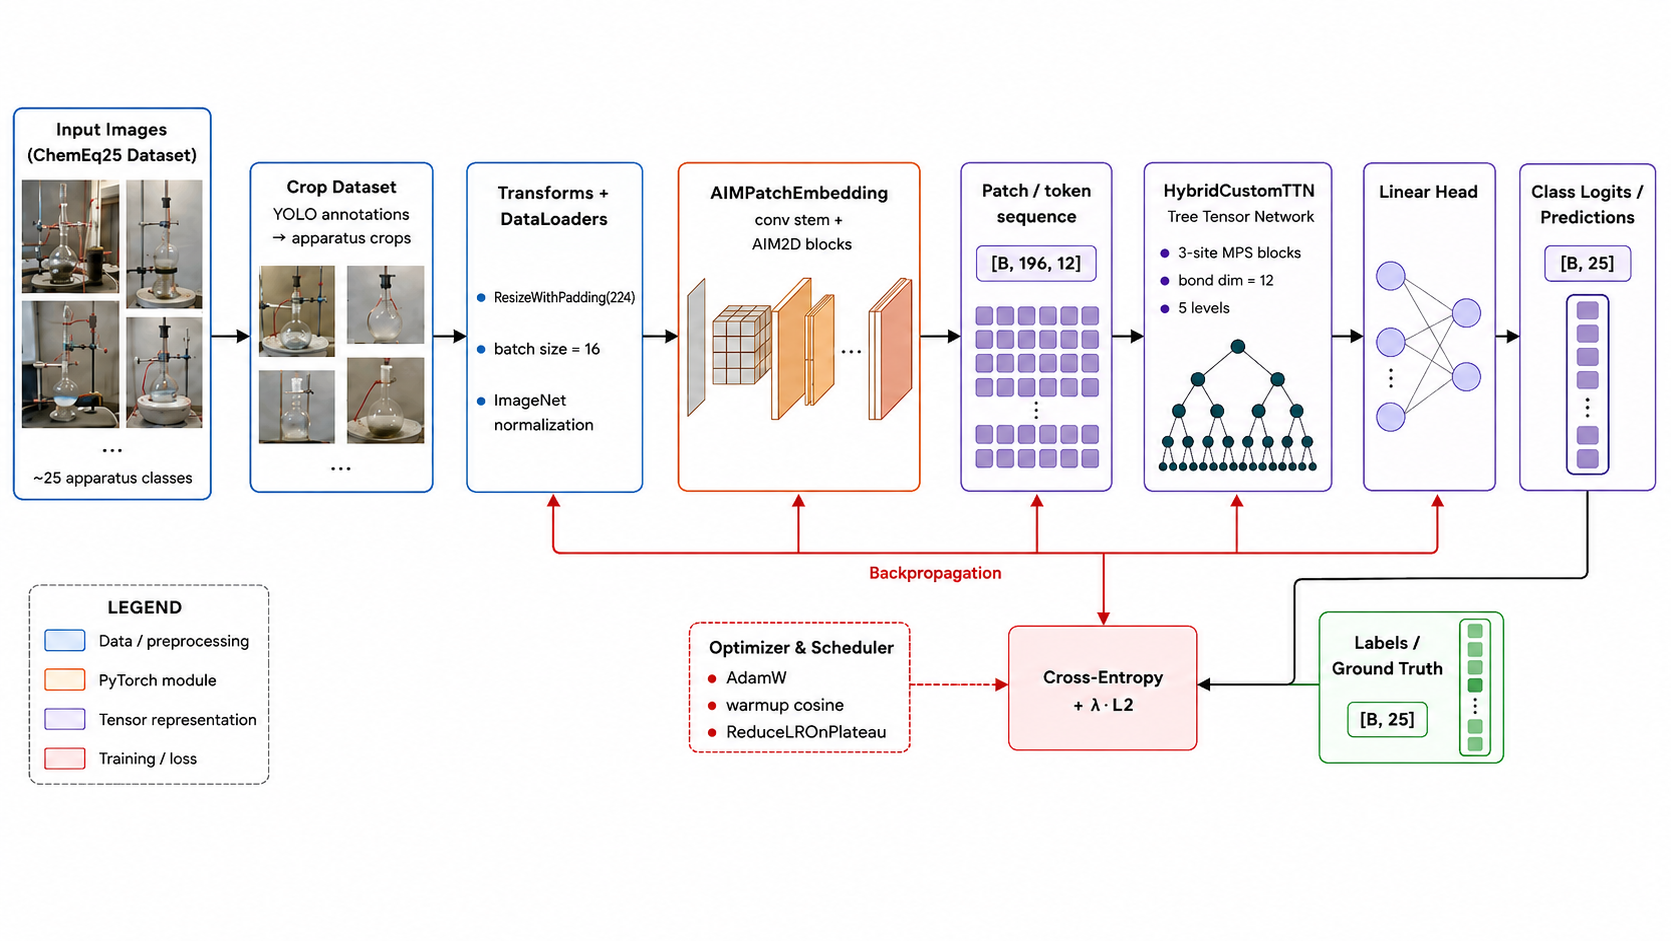
\includegraphics[width=1.0\linewidth]{figures/Pipeline_Scheme.png}
    \caption[Esquema general del pipeline]{Esquema general del pipeline desarrollado en el trabajo. A partir de las imágenes originales y sus anotaciones se generan recortes individuales de objetos, se aplican transformaciones y se agrupan en lotes. Cada imagen procesada entra en la etapa de \textit{embedding}, que produce una secuencia compatible con la red tensorial. La salida de la red tensorial pasa por una cabeza de clasificación y se compara con la etiqueta real mediante la función de pérdida. Las flechas inferiores representan la actualización de parámetros por retropropagación.}
    \label{fig:pipeline_scheme}
\end{figure}

El código del proyecto se organizó de forma modular, separando responsabilidades en distintos módulos diferenciados. Esta organización hace que el proyecto sea mucho más manejable y permite modificar una parte sin alterar el resto. El detalle de la estructura de carpetas se recoge en los anexos.

Por último, cada configuración de los experimentos queda definida por un archivo de configuración en formato YAML (\textit{Yet Another Markup Language}), que fija todos los parámetros relevantes, como el conjunto de datos, el tamaño de imagen, el tipo de \textit{embedding}, la dimensión local y la dimensión de enlace, el número de épocas, el ritmo de aprendizaje, la regularización, el \textit{scheduler} y la semilla aleatoria, entre otros. De este modo, un experimento puede repetirse o compararse leyendo simplemente su configuración, sin depender de notas externas. Esta forma de trabajar es la base de la trazabilidad del proyecto.

\section{Preparación del dataset ChemEq25}

El dataset utilizado en este proyecto es ChemEq25, también llamado en el código \textit{Chemistry Lab Apparatus} \citebox{hossain2025chemistrylabdataset}. Este dataset contiene imágenes de material de laboratorio y anotaciones asociadas a los objetos presentes en cada imagen.

El problema no se trató como una clasificación directa de imágenes completas debido a que, en muchas imágenes aparece más de un objeto, y esos objetos pueden pertenecer a clases distintas. Si se introdujera la imagen completa en el clasificador, la etiqueta sería ambigua. Por eso se reformuló el problema como clasificación por instancia, en el que cada anotación YOLO (\textit{You Only Look Once}) genera un recorte o \textit{crop} de un único objeto, y ese crop se asocia a una clase.

Tras convertir las anotaciones en muestras individuales, los tamaños de los splits fueron:

\begin{center}
\begin{tabular}{c|c}
\textbf{Split} & \textbf{Número de crops} \\
\hline
Entrenamiento & 4863 \\
Validación & 1393 \\
Test & 704 \\
\end{tabular}
\end{center}

El procedimiento de lectura e interpretación (\textit{parser} en inglés) de las anotaciones tuvo que contemplar dos casos. Algunas etiquetas seguían el formato YOLO habitual:

\begin{center}
\texttt{class\_id x\_center y\_center width height}
\end{center}

pero otras contenían más coordenadas, correspondientes a polígonos de segmentación. Para que todo pudiera tratarse de manera uniforme, las anotaciones de cinco coordenadas se interpretaron como cajas YOLO y las anotaciones con más coordenadas se transformaron en la caja rectangular envolvente del polígono.

Después de obtener el \textit{crop}, todas las imágenes deben convertirse a un tamaño común para entrar al modelo. Inicialmente se podía usar un \texttt{Resize(224, 224)} directo, pero esto deforma objetos alargados como pipetas, tubos de ensayo o varillas. Por esa razón se implementó una opción para preservar la relación de aspecto y rellenar hasta obtener una imagen cuadrada. El color de relleno se escogió cercano a la media de \textit{ImageNet}, de forma que tras la normalización el relleno (\textit{padding}) no quedara como un borde artificial demasiado dominante.

\section{Transformaciones y aumento de datos}

El preprocesamiento de las imágenes se separó entre entrenamiento y evaluación. La parte de evaluación consta de un proceso de validación y otro de test. En esta parte no se aplican transformaciones aleatorias, porque se quiere medir el comportamiento del modelo sobre datos estables. En el entrenamiento sí se usa \textit{data augmentation}, con el objetivo de que el modelo no memorice una única apariencia de cada objeto.

Este proceso de aumento de datos se hizo configurable, es decir, que el usuario puede decidir si quiere aplicarlo o no. En ChemEq se usaron opciones como:

\begin{itemize}
    \item \texttt{augmentation\_name = none}, sin aumentos aleatorios.
    \item \texttt{augmentation\_name = basic}, con transformaciones suaves ya existentes.
    \item \texttt{augmentation\_name = light}, añadiendo rotaciones pequeñas y \texttt{RandomErasing} bajo.
\end{itemize}

La configuración final más relevante usó la configuración \texttt{light}, rotaciones de 7 grados y \texttt{RandomErasing} con probabilidad 0,10. La idea fue introducir variabilidad sin destruir la geometría del objeto, porque en material de laboratorio la forma es precisamente una parte importante de la clase.

\section{Representación de la imagen como secuencia}

Una red tensorial no procesa directamente una imagen con forma \texttt{[C, H, W]} (canales, alto y ancho). Su entrada natural es una secuencia ordenada de vectores locales. Dicho de otra forma, son un conjunto de posiciones de entrada en el que cada posición aporta un vector de dimensión fija. Por eso, antes de la red tensorial es necesaria una etapa que transforme la imagen en esa secuencia:

\begin{center}
\texttt{[B, C, H, W] -> [B, L, local\_dim]}
\end{center}

donde \texttt{B} es el número de imágenes que se procesan a la vez (un \textit{batch} o lote), \texttt{L} es el número de posiciones de entrada de la red tensorial y \texttt{local\_dim} es la dimensión del vector asociado a cada posición. Esta etapa se denomina \textit{embedding} de la imagen y es una parte muy importante del modelo, ya que condiciona su rendimiento de manera considerable, porque determina qué información espacial llega a la red tensorial y en qué forma se le entrega.

El primer enfoque que se probó dividía la imagen en cuadrados y proyectaba cada uno de forma independiente con una transformación lineal. Este enfoque resultó insuficiente, ya que al construir la secuencia se pierde la estructura bidimensional de la imagen y la relación de vecindad entre cuadrados contiguos. Por ese motivo, la versión final del proyecto utiliza un \textit{embedding} que conserva la estructura espacial hasta el último momento, denominado en el código \texttt{AIMPatchEmbedding}. A continuación se describe su funcionamiento.

El \texttt{AIMPatchEmbedding} no trocea la imagen, sino que la procesa como un mapa bidimensional que se va reduciendo de tamaño progresivamente. Solo en el último paso ese mapa se aplana para formar la secuencia que recibe la red tensorial. El flujo completo de dimensiones, para imágenes de entrada de $224\times224$, es:

\begin{center}
\texttt{[B, 3, 224, 224]} \\
\texttt{-> stem convolucional -> [B, C\_aim, 14, 14]} \\
\texttt{-> bloques AIM -> [B, C\_aim, 14, 14]} \\
\texttt{-> convolución 1x1 -> [B, local\_dim, 14, 14]} \\
\texttt{-> aplanado + zigzag -> [B, 196, local\_dim]}
\end{center}

La imagen pasa primero por un bloque convolucional inicial, denominado habitualmente \textit{stem}, cuya función es extraer características locales básicas y reducir la resolución espacial de la entrada. Después por una serie de bloques AIM que mantienen el mapa espacial e introducen interacciones entre canales y posiciones, y finalmente por una proyección que ajusta el número de canales a la dimensión local que espera la red tensorial. El mapa resultante de $14\times14$ se aplana en una secuencia de $196$ posiciones de entrada.

El \textit{stem} es la etapa inicial que sustituye el corte en cuadrados por una pequeña red convolucional. Una convolución es una operación que desliza un filtro pequeño sobre la imagen para detectar patrones locales (bordes, texturas, formas) reutilizando los mismos pesos en todas las posiciones. El \textit{stem} se construye como una pila de bloques, cada uno formado por una convolución con paso (\textit{stride}) dos, seguida de una normalización por lotes (\textit{BatchNorm}, que reescala las activaciones usando estadísticas del propio \textit{batch} para estabilizar el entrenamiento) y una función de activación ReLU (que anula los valores negativos e introduce no linealidad).

El paso dos significa que el filtro se desplaza de dos en dos píxeles, de modo que cada bloque reduce a la mitad el alto y el ancho del mapa. El número de bloques viene dado por el hiperparámetro \texttt{patch\_size}, que en este \textit{embedding} ya no representa el tamaño de un cuadrado, sino el factor total de reducción espacial. Debe ser una potencia de dos, y el número de bloques es $\log_2(\texttt{patch\_size})$. Con \texttt{patch\_size = 16} se encadenan cuatro bloques, que reducen la imagen de la siguiente forma:

\begin{center}
\texttt{224 -> 112 -> 56 -> 28 -> 14}
\end{center}

El primer bloque transforma los tres canales de color en \texttt{aim\_channels} canales, y los siguientes mantienen ese número. El resultado es un mapa \texttt{[B, aim\_channels, 14, 14]} en el que cada una de las $14\times14$ posiciones del mapa pasará a ser una posición de entrada de la red tensorial.

Sobre el mapa producido por el \textit{stem} se aplican uno o varios bloques AIM, inspirados en el trabajo \textit{Deep Tree Tensor Networks for Image Recognition} \citebox{nie2025deeptreetensornetworks}. Cada bloque recibe un mapa \texttt{[B, C, H, W]} y devuelve otro de la misma forma, lo que permite encadenar varios y, como se verá, añadir una conexión residual.

La idea central del bloque es construir dos ramas que aplican las mismas dos familias de operaciones, pero en orden inverso:

\begin{itemize}
    \item \textbf{Rama 1:} primero una transformación lineal que mezcla los canales en cada píxel y una convolución que aplica un filtro espacial independiente a cada canal sin mezclar información entre canales.
    \item \textbf{Rama 2:} primero una convolución agrupada (\textit{grouped}), que procesa cada canal de entrada por separado para generar varios canales nuevos, y después una transformación lineal que mezcla los canales.
\end{itemize}

Internamente ambas ramas expanden el número de canales por un factor configurable (\texttt{expansion\_ratio}), lo que da al bloque más capacidad de representación antes de volver a comprimir. Las salidas de las dos ramas se combinan mediante un producto de Hadamard, esto es, una multiplicación elemento a elemento de dos tensores de la misma forma:

\begin{center}
\texttt{interaction = f1(x) * f2(x)}
\end{center}

Este producto es la clave del bloque y el motivo por el que encaja bien delante de una red tensorial. Las dos ramas se construyen sin término independiente (\textit{bias}) y sin funciones de activación intermedias, de modo que cada una es una transformación lineal de la entrada. Al multiplicarlas elemento a elemento, el resultado es bilineal, es decir, cuadrático en la entrada. Se introduce así una interacción multiplicativa entre las características de la imagen, justo el tipo de operación que las redes tensoriales expresan de forma natural, y sin recurrir a no linealidades del tipo ReLU o sigmoide. El nombre del módulo en la literatura, \textit{Antisymmetric Interaction Module} (AIM), alude precisamente a esa construcción en orden inverso de las dos ramas antes del producto.

Tras el producto, el resultado se normaliza con una normalización por capas (\textit{LayerNorm}, que reescala cada vector de canales para estabilizar su escala y distribución) y se proyecta de vuelta al número original de canales mediante una convolución $1\times1$, de manera que la salida pueda sumarse con la entrada del bloque. Esta suma es una conexión residual; en lugar de reemplazar la entrada, el bloque aprende una corrección que se le añade,

\begin{center}
\texttt{salida = x + s * correccion}
\end{center}

donde \texttt{s} es un factor de escala entrenable inicializado a un valor pequeño. Inicializarlo pequeño hace que, al comienzo del entrenamiento, el bloque se comporte casi como la identidad y no desestabilice las activaciones que recibirá la red tensorial. La etapa AIM aplica \texttt{num\_aim\_blocks} bloques de este tipo de forma consecutiva.

Después de los bloques AIM, una última convolución $1\times1$ ajusta el número de canales desde \texttt{aim\_channels} hasta \texttt{local\_dim}, la dimensión que espera la red tensorial en cada posición. El mapa resultante, de forma \texttt{[B, local\_dim, 14, 14]}, se reordena para situar los canales al final y se aplana convirtiendo la rejilla espacial en una secuencia:

\begin{center}
\texttt{[B, local\_dim, 14, 14] -> [B, 196, local\_dim]}
\end{center}

El orden en que se recorren las $196$ posiciones no es indiferente. Un recorrido por filas (\textit{row-major}) saltaría del final de una fila al principio de la siguiente, introduciendo una discontinuidad espacial entre posiciones consecutivas de la secuencia. Para suavizar este efecto se emplea un recorrido en zigzag. Las filas pares se recorren de izquierda a derecha y las impares de derecha a izquierda, de modo que dos posiciones contiguas en la secuencia tienden a ser también vecinas en la imagen. Cada una de las $196$ posiciones resultantes es un vector local de dimensión \texttt{local\_dim} y constituye una posición de entrada de la red tensorial descrita en la siguiente sección.

\medskip

En conjunto, este \textit{embedding} conserva la estructura espacial bidimensional de la imagen hasta el momento mismo del aplanado, en lugar de destruirla al inicio. Las convoluciones, al compartir pesos entre posiciones, actúan como un sesgo inductivo y como una forma de regularización, y la interacción multiplicativa del bloque AIM aporta una no linealidad coherente con el lenguaje de las redes tensoriales. La conexión residual, por su parte, permite que la etapa inicial parta de un comportamiento próximo a la identidad y estabilice el entrenamiento del modelo completo.

\section{Arquitectura tensorial propuesta}\label{sec:arquitectura}

La secuencia de $196$ vectores locales producida por el \textit{embedding} es la entrada de la red tensorial entrenable, que procesa la información hasta obtener un único vector con el que se decide la clase. El tipo de red tensorial es una jerárquica de tipo \textit{Tree Tensor Network} (TTN), denominada en el código \texttt{HybridCustomTTN}, que se describe a continuación.

La idea de una TTN es organizar el cálculo como un árbol. Las posiciones de entrada se agrupan de tres en tres, cada grupo se contrae con un pequeño bloque tensorial que produce un solo vector de salida, y ese vector pasa a ser una entrada del siguiente nivel del árbol. El proceso se repite, reduciendo el número de posiciones en cada nivel, hasta llegar a un único vector raíz que resume toda la imagen. Que los grupos sean de tres elementos es lo que se denomina aridad tres del árbol.

\begin{figure}[H]
    \centering
    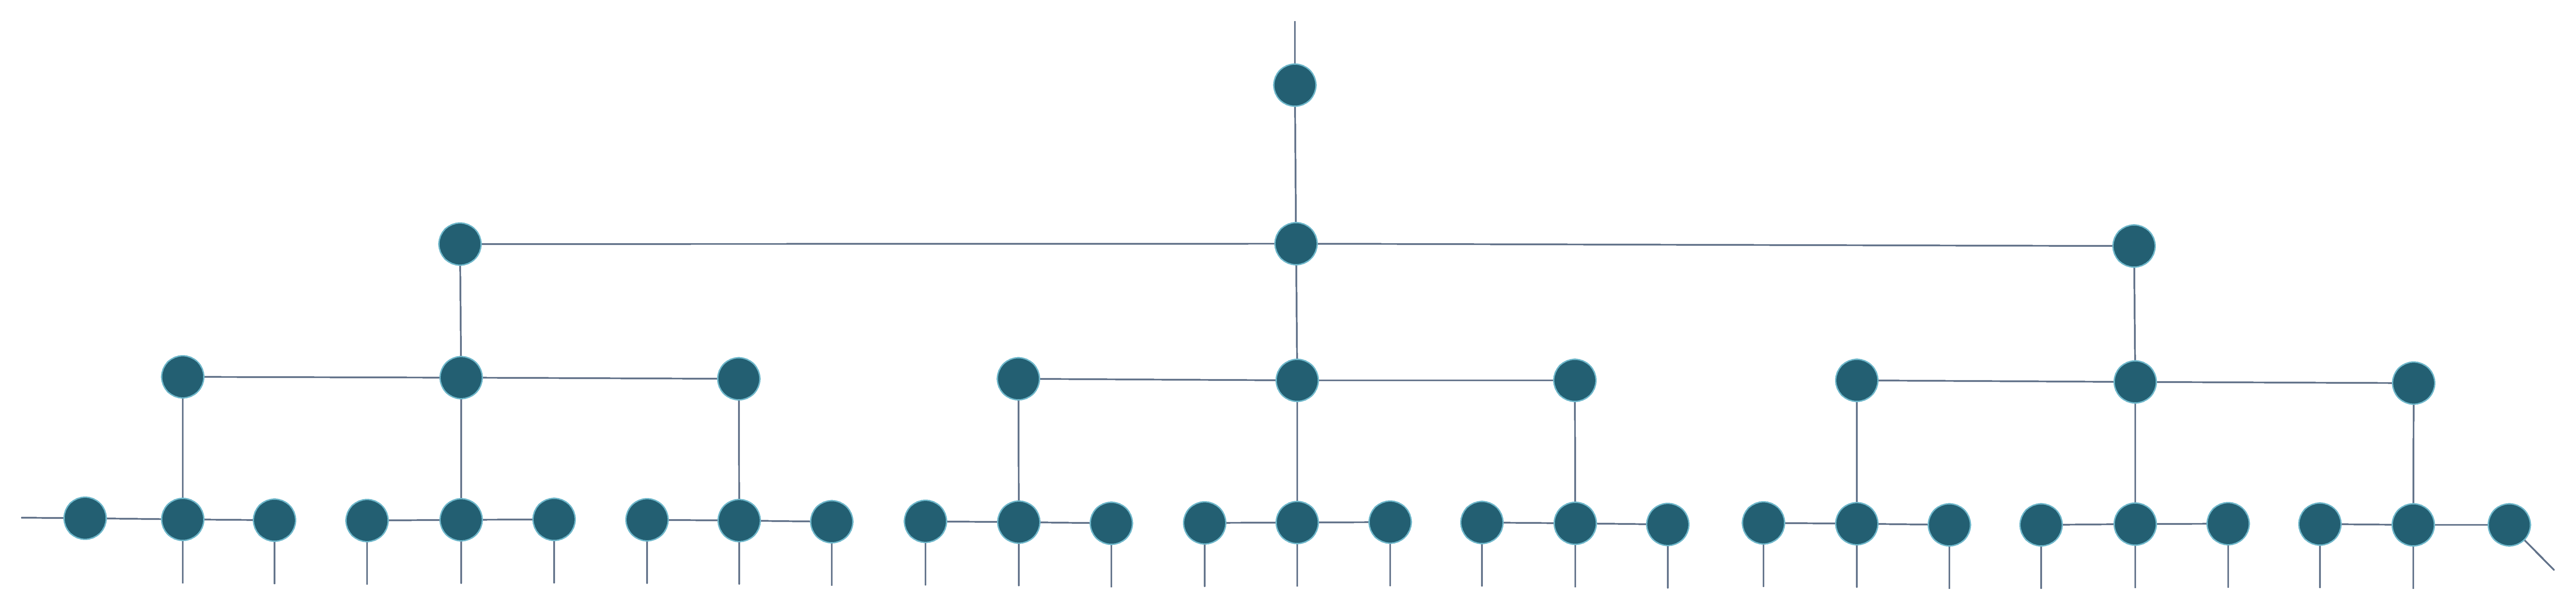
\includegraphics[width=1\linewidth]{figures/ttn_model.pdf}
    \caption[Diagrama de la \textit{Tree Tensor Network} propuesta]{Diagrama de la TTN. Es una imagen orientativa, ya que representa tres niveles cuando la arquitectura empleada tiene cinco. Las posiciones de entrada se agrupan de tres en tres y se contraen jerárquicamente hasta un único vector raíz. Imagen de elaboración propia con la librería Tensor-Network-Editor, creada por Alejandro Mata Ali. \citebox{Mata_Ali_Tensor_Network_Editor_2026}}
    \label{fig:ttn_diagram}
\end{figure}

En el lenguaje de redes tensoriales conviene distinguir dos tipos de índices. Los índices físicos (o de entrada) son los que conectan la red con los datos; por cada posición de entrada hay un índice físico cuya dimensión es la del vector local que llega a esa posición. En el primer nivel esa dimensión es \texttt{local\_dim}, la que produce el \textit{embedding}. Los índices virtuales (o de enlace) son internos; conectan unos tensores con otros dentro de la red y no tocan los datos. Su dimensión común se denomina dimensión de enlace (\texttt{bond\_dim}).

La dimensión de enlace es el principal parámetro que controla la capacidad del modelo. Cuanto mayor es \texttt{bond\_dim}, más información puede transmitirse a través de cada conexión interna y más ricas son las correlaciones que la red puede representar entre distintas partes de la imagen, a costa de más parámetros y más coste de cálculo. Junto con la topología del árbol, es la decisión de diseño que regula el equilibrio entre capacidad y eficiencia.

La unidad básica de la TTN es un bloque tensorial de tres nodos, con la estructura de una MPS corta. Cada bloque está formado por un nodo izquierdo, uno central y uno derecho. El nodo izquierdo tiene un índice físico de entrada y un índice virtual que lo une al central. El nodo central tiene un índice físico de entrada, dos índices virtuales (uno hacia el nodo izquierdo y otro hacia el derecho) y un índice de salida. El nodo derecho tiene un índice físico de entrada y un índice virtual que lo une al central.

El índice de salida se sitúa en el nodo central y tiene dimensión \texttt{bond\_dim}; es el que conecta el bloque con el nivel superior del árbol. Cada bloque recibe tres vectores de entrada (uno por nodo) y los contrae junto con sus tres tensores para producir un único vector de salida. Si se denota por $v^{(1)}, v^{(2)}, v^{(3)}$ a los tres vectores de entrada, por $A$, $C$ y $B$ a los tensores de los nodos izquierdo, central y derecho, y se usan las letras $a,b$ para los índices virtuales, $i,j,k$ para los físicos y $\beta$ para el de salida, la salida del bloque es:

\begin{equation}
o_{\beta} \;=\; \sum_{a,b}\;\sum_{i,j,k} A_{a\,i}\, C_{a\,b\,j\,\beta}\, B_{b\,k}\; v^{(1)}_{i}\, v^{(2)}_{j}\, v^{(3)}_{k}.
\end{equation}

Los índices virtuales $a$ y $b$ tienen dimensión \texttt{bond\_dim}, los físicos $i,j,k$ tienen la dimensión de entrada del nivel y el índice de salida $\beta$ tiene de nuevo dimensión \texttt{bond\_dim}. La contracción combina de forma multiplicativa la información de los tres vectores de entrada, lo que conecta directamente con la motivación de usar redes tensoriales. La salida depende de productos entre las componentes de la entrada, no solo de sumas ponderadas.

Los tres tensores de cada bloque son parámetros entrenables del modelo. En la implementación esto exigió declararlos de un tipo específico de TensorKrowch (\texttt{ParamNode}), de modo que sus valores se registran como parámetros del modelo y reciben gradientes durante el entrenamiento; si se hubieran creado como nodos ordinarios, no aparecerían como parámetros entrenables. Sus valores se inicializan con ruido aleatorio de desviación típica pequeña ($0{,}02$), un valor que mantiene las contracciones numéricamente estables a medida que se asciende por los niveles del árbol.

El número de posiciones de un nivel no siempre es múltiplo de tres. Cuando el último grupo queda incompleto, las posiciones que faltan se rellenan con nodos constantes, no entrenables, cuyo vector es $[1, 0, \dots, 0]$. Estos nodos de relleno (\textit{padding}) completan el grupo para que el bloque pueda contraerse, pero no aportan parámetros ni introducen información, ya que su vector es fijo y neutro. De esta forma la estructura jerárquica se mantiene regular sin distorsionar el aprendizaje.

Cada nivel del árbol se implementó como una red tensorial independiente (\texttt{TTNLevel}) que contrae únicamente su propio nivel de bloques de tres nodos y devuelve un tensor de PyTorch ordinario. El enlace entre un nivel y el siguiente no se hace dentro de TensorKrowch, sino en PyTorch: la salida de un nivel, antes de entrar en el siguiente, pasa por una pequeña transformación estándar formada por una normalización por capas (\textit{LayerNorm}), una capa lineal y una activación ReLU:

\begin{center}
\texttt{nivel -> LayerNorm -> Linear -> ReLU -> nivel siguiente}
\end{center}

Esta combinación es la razón del nombre \texttt{HybridCustomTTN}. Es híbrida porque las contracciones tensoriales se realizan con TensorKrowch, mientras que las transformaciones intermedias, el entrenamiento y la integración del modelo se gestionan con PyTorch. Las transformaciones entre niveles aportan flexibilidad adicional y ayudan a estabilizar las escalas de los vectores al pasar de un nivel a otro.

Partiendo de las $196$ posiciones de entrada y agrupando de tres en tres, el número de posiciones se reduce nivel a nivel de la forma

\begin{center}
\texttt{196 -> 66 -> 22 -> 8 -> 3 -> 1},
\end{center}

de modo que la arquitectura empleada consta de cinco niveles tensoriales y cuatro transformaciones intermedias. La salida del último nivel es un único vector raíz de dimensión \texttt{bond\_dim} que condensa la información de toda la imagen.

El vector raíz no es todavía una predicción. Para obtener una puntuación por clase se aplica una cabeza de clasificación, que en su versión más sencilla es una única capa lineal que transforma el vector raíz de dimensión \texttt{bond\_dim} en un vector de dimensión igual al número de clases ($25$ en ChemEq25). Las componentes de ese vector son las puntuaciones sin normalizar de cada clase (\textit{logits}), que en la etapa de entrenamiento se compararán con la etiqueta real mediante la función de pérdida descrita más adelante. Opcionalmente, esta cabeza puede sustituirse por un pequeño perceptrón multicapa con una capa oculta, una activación y regularización por \textit{dropout}, aunque la versión lineal es la que define el modelo de referencia.

\section{Entrenamiento y regularización}\label{sec:entrenamiento}

Una vez definidos el \textit{embedding} y la red tensorial, el modelo se entrena ajustando sus parámetros para que clasifique correctamente los recortes. En cada paso, el modelo procesa un \textit{batch} de imágenes y produce sus puntuaciones por clase; una función de pérdida mide cuánto se equivoca, y a partir de ese error se calculan los gradientes que indican cómo modificar cada parámetro para reducirlo. Esta sección explica las decisiones tomadas en ese proceso: la función de pérdida, las técnicas de regularización y el control del ritmo de aprendizaje.

Para entrenar el clasificador se empleó la entropía cruzada, una función de pérdida habitual en problemas de clasificación con varias clases. El modelo no devuelve directamente probabilidades, sino una puntuación para cada clase (los \textit{logits} introducidos antes). Durante el cálculo de la pérdida, esas puntuaciones se transforman internamente en probabilidades normalizadas y se penaliza al modelo cuando asigna una probabilidad baja a la clase correcta. Cuanto más confiado está el modelo en la clase verdadera, menor es la pérdida.

En la implementación, esta función (\texttt{CrossEntropyLoss} en PyTorch) combina internamente la normalización en probabilidades (\textit{softmax}) y la comparación con la etiqueta correcta. Por eso el modelo no necesita aplicar esa normalización en su capa de salida, basta con que produzca los \textit{logits}. Esta combinación interna evita duplicar operaciones y hace el entrenamiento numéricamente más estable.

Durante el entrenamiento se aplicó además un suavizado de etiquetas (\textit{label smoothing}). En lugar de exigir al modelo que asigne toda la probabilidad a la clase correcta y exactamente cero al resto, el objetivo se relaja ligeramente, dejando una pequeña parte de probabilidad repartida entre las demás clases. Esto evita que el modelo se vuelva excesivamente confiado y suele mejorar su capacidad de generalizar a imágenes nuevas.

El suavizado solo se usa en entrenamiento. En la evaluación se emplea la entropía cruzada normal, sin suavizado, de modo que la pérdida de validación (\texttt{eval\_loss}) sigue midiendo el ajuste real del modelo frente a las etiquetas verdaderas y permite comparar experimentos de forma coherente.

El optimizador es el algoritmo que decide cómo actualizar los parámetros del modelo a partir de los gradientes. Se utilizó AdamW (\texttt{AdamW}), una variante muy extendida del optimizador Adam. Adam adapta automáticamente el tamaño del paso de actualización para cada parámetro, usando estimaciones del comportamiento reciente de sus gradientes, lo que suele acelerar y estabilizar el entrenamiento frente a un descenso de gradiente simple. La variante AdamW incorpora además, de forma adecuada, una penalización que tiende a mantener pequeños los pesos del modelo (\textit{weight decay}), descrita a continuación.

La regularización agrupa las técnicas que evitan que el modelo se limite a memorizar las imágenes de entrenamiento (sobreajuste) en lugar de aprender características que generalicen. En este trabajo se combinaron dos mecanismos. El primero es la penalización por reducción de pesos (\textit{weight decay}) que incorpora AdamW, que empuja suavemente los pesos hacia valores pequeños. El segundo es una penalización L2 explícita y configurable. Durante el entrenamiento se añade a la pérdida un término proporcional a la suma de los cuadrados de los pesos del modelo. Esta penalización se aplica solo a las matrices de pesos, excluyendo los términos independientes y los parámetros de las capas de normalización, que no conviene penalizar de la misma forma.

Un detalle importante de trazabilidad es que, aunque este término de regularización se suma a la pérdida que guía la actualización de los parámetros, la métrica registrada como \texttt{train\_loss} conserva únicamente la entropía cruzada. De este modo, la pérdida de entrenamiento y la de validación miden lo mismo y son directamente comparables entre sí y entre experimentos.

El ritmo de aprendizaje (\textit{learning rate}) determina cómo de grandes son los pasos con los que se actualizan los parámetros en cada iteración. Un valor demasiado grande puede hacer que el entrenamiento se vuelva inestable; uno demasiado pequeño lo ralentiza. Para gestionarlo se combinaron dos mecanismos.

El primero es un calentamiento inicial (\textit{warmup}). Durante las primeras épocas, el ritmo de aprendizaje no parte de su valor máximo, sino que crece de forma gradual, ya sea de manera lineal o siguiendo un perfil más suave, hasta alcanzar el valor objetivo. Empezar con pasos pequeños evita las grandes oscilaciones que pueden producirse al inicio, cuando los parámetros aún están lejos de una buena solución.

El segundo mecanismo actúa una vez terminado el calentamiento: el ritmo de aprendizaje se reduce automáticamente cuando la pérdida de validación deja de mejorar durante varias épocas seguidas (\texttt{ReduceLROnPlateau}). La idea es dar pasos más finos a medida que el modelo se acerca a una solución y ya no progresa con el ritmo anterior. La implementación contempla también, como alternativa, un descenso suave y continuo del ritmo de aprendizaje a lo largo del entrenamiento (\textit{cosine decay}).

Finalmente, el estado del optimizador y del controlador del ritmo de aprendizaje se guarda junto con el mejor modelo en cada punto de control (\textit{checkpoint}). Esto permite reanudar un entrenamiento interrumpido exactamente en las mismas condiciones en que se dejó, lo que resultó útil para los entrenamientos largos ejecutados en el servidor.

\section{Métricas, diagnósticos y trazabilidad}

Cada entrenamiento genera una carpeta dentro de \texttt{runs/}. En ella se guardan la configuración resuelta, el checkpoint del mejor modelo, el archivo \texttt{metrics.csv}, las curvas de pérdida y los diagnósticos. Esto fue fundamental para poder reconstruir qué se había probado y con qué parámetros.

En cada época se registran en \texttt{metrics.csv} varias métricas que resumen el comportamiento del modelo sobre el conjunto de entrenamiento y sobre el de validación. La primera es la pérdida (\texttt{train\_loss} y \texttt{eval\_loss}), que mide cómo de lejos queda la predicción de la respuesta correcta. Cuanto más baja es, mejor es el ajuste, y penaliza especialmente los fallos cometidos con mucha seguridad. La versión \texttt{train} se calcula sobre los datos de entrenamiento y la \texttt{eval} sobre los recortes de validación, que el modelo no ha visto durante el ajuste. A continuación está el acierto o \textit{accuracy} top-1 (\texttt{train\_accuracy} y \texttt{eval\_accuracy}), que es la fracción de recortes en los que la clase más probable para el modelo coincide con la real; es la medida más directa de rendimiento, de modo que un valor de 0,96 indica que el modelo acierta la primera predicción en el 96\% de los casos. El acierto top-5 (\texttt{eval\_top5\_accuracy}) es una versión más permisiva; cuenta los recortes en los que la clase correcta está entre las cinco más probables, aunque no sea la primera, y sirve para ver si el modelo se acerca a la respuesta correcta cuando su primera elección falla. Por último, la confianza media en aciertos y en errores (\texttt{mean\_confidence\_correct} y \texttt{mean\_confidence\_wrong}) recoge la probabilidad que el modelo asigna a la clase que elige; al promediarla por separado según acierte o falle, se puede comprobar si está bien calibrado o si se equivoca con demasiada seguridad.

Al terminar cada entrenamiento, a partir del mejor checkpoint se calculan además métricas por clase sobre el conjunto de validación. La precisión (\textit{precision}) de una clase indica, de todos los recortes que el modelo asigna a ella, qué fracción le pertenece realmente, por lo que penaliza los falsos positivos. La exhaustividad (\textit{recall}) indica, de todos los recortes que pertenecen de verdad a esa clase, qué fracción consigue recuperar el modelo, por lo que penaliza los que se le escapan. El F1 combina ambas en su media armónica, que da más peso al menor de los dos valores, de manera que solo es alto cuando la precisión y la exhaustividad lo son a la vez. Para resumir el rendimiento global se usa la media macro de estas tres métricas, es decir, el promedio simple sobre las 25 clases dando el mismo peso a cada una con independencia de cuántos recortes contenga, lo que evita que las clases más numerosas dominen el resultado.

Junto a estas métricas se generan otros diagnósticos, como la matriz de confusión, la distribución de predicciones, las principales confusiones, las curvas \textit{precision-recall} y las curvas F1-confianza. La matriz de confusión es especialmente útil, ya que sus filas representan la clase real y sus columnas la clase predicha, de modo que la diagonal recoge los aciertos y los valores fuera de ella muestran entre qué clases se confunde el modelo. En este TFG todas estas métricas se interpretan como métricas de clasificación de recortes, una distinción importante porque el paper de ChemEq25 evalúa modelos de detección, mientras que aquí el modelo clasifica recortes ya generados a partir de las anotaciones, sin localizar cajas ni medir solapamientos.

\section{Comparación con ResNet50}\label{sec:resnet}

Para situar el rendimiento de la arquitectura tensorial dentro de un marco más amplio, se incorporó como referencia una arquitectura convolucional estándar de visión artificial; ResNet50. El objetivo de esta comparación no es demostrar que un modelo supere al otro, sino contextualizar los resultados de la red tensorial frente a un modelo ampliamente utilizado y bien comprendido, e identificar qué decisiones de diseño influyen más en el rendimiento.

La comparación se diseñó para ser justa, en el sentido de aislar el efecto de la arquitectura. ResNet50 clasifica exactamente los mismos recortes que la red tensorial. Se utilizan las mismas particiones de entrenamiento, validación y test, las mismas $25$ clases de ChemEq25 y la misma normalización de las imágenes (con la media y la desviación típica de ImageNet que ya produce la preparación de datos). Además, ambos modelos comparten el mismo bucle de entrenamiento y evaluación y se valoran con las mismas métricas. De este modo, la principal diferencia controlada entre los experimentos es la arquitectura del modelo.

El modelo se tomó de la librería \texttt{torchvision}, sustituyendo únicamente su capa final de clasificación por una capa lineal hacia las $25$ clases del problema (con la opción de añadir regularización por \textit{dropout}). Sobre esta base se evaluaron dos esquemas de entrenamiento, que se corresponden con dos formas distintas de inicializar los pesos del modelo:

\begin{itemize}
    \item \textbf{Entrenamiento desde cero.} La red parte de pesos aleatorios y aprende únicamente a partir de los recortes de ChemEq25, sin ningún conocimiento previo. Sirve como referencia de cuánto puede aprender la arquitectura con los datos disponibles del problema.

    \item \textbf{Ajuste fino.} La red parte de pesos preentrenados sobre ImageNet, un gran conjunto de imágenes de uso general, y todos sus pesos se actualizan durante el entrenamiento, ajustando las características visuales generales aprendidas previamente al problema concreto de material de laboratorio. Constituye la referencia más habitual y fuerte de visión artificial.
\end{itemize}

En la implementación, ambos esquemas se controlan con una opción de configuración que indica si se parte de pesos preentrenados sobre ImageNet o de pesos aleatorios. Cada esquema se entrenó con una tasa de aprendizaje distinta según su inicialización. Para el modelo entrenado desde cero se empleó un valor mayor, mientras que para el modelo preentrenado se utilizó un valor menor durante el ajuste fino, con el objetivo de adaptar sus pesos al nuevo problema sin modificar bruscamente las características ya aprendidas. Estos experimentos de referencia incorporaron además un criterio de parada temprana (\textit{early stopping}), que detiene el entrenamiento cuando la pérdida de validación deja de mejorar durante un número fijo de épocas, evitando épocas innecesarias una vez alcanzado el mejor rendimiento. Los resultados cuantitativos de cada esquema, junto con su comparación con la red tensorial propuesta, se presentan y discuten en el capítulo de resultados.

\section{Reproducibilidad y ejecución en servidor}\label{sec:reproducibilidad}

Todos los entrenamientos se ejecutaron en los servidores Lorca de la universidad. El uso de estos recursos forma parte de la metodología del proyecto, porque permitió lanzar experimentos largos, aprovechar la aceleración por GPU, guardar puntos de control y analizar las métricas con posterioridad.

\begin{figure}[H]
    \centering
    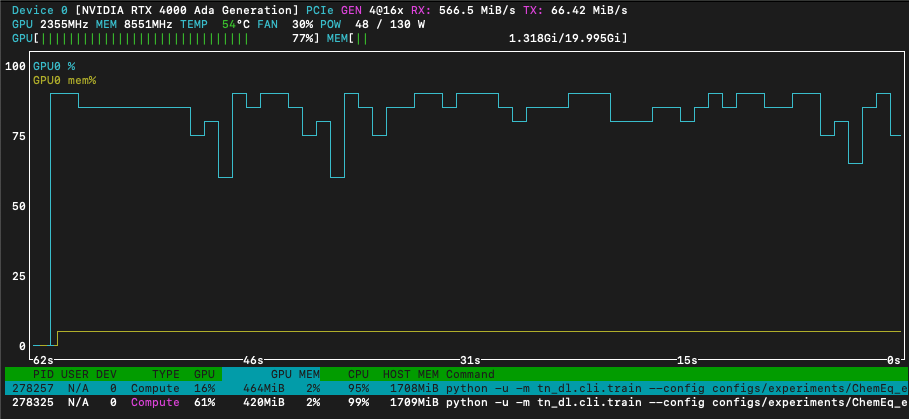
\includegraphics[width=1.0\linewidth]{figures/GPU_picture.png}
    \caption{Captura de una GPU NVIDIA RTX 4000 Ada Generation del servidor Lorca de la UEM ejecutando dos procesos de entrenamiento en paralelo.}
    \label{fig:gpu_lorca}
\end{figure}

El trabajo en el servidor obligó a cuidar el entorno de Python, las dependencias y los scripts de lanzamiento, así como a registrar de forma ordenada los resultados de cada ejecución. Esto fue especialmente importante porque muchas pruebas se lanzaron en paralelo o en días distintos; sin un registro fiable habría sido difícil distinguir si una mejora provenía de la arquitectura, del preprocesamiento, de la semilla aleatoria, del ritmo de aprendizaje o de la regularización.

La reproducibilidad se cuidó de forma explícita. Cada ejecución fija una semilla aleatoria, lo que hace que el entrenamiento sea repetible, y conserva la configuración resuelta y las métricas ya descritas, de modo que un experimento puede reconstruirse a partir de esos archivos sin depender de notas externas. El código completo del proyecto está disponible en un repositorio público enlazado en los anexos, donde se incluye también una nota con las instrucciones necesarias para reproducir los experimentos.